
%\documentclass{cmspaper}
%\begin{document}

\section{Monte Carlo Samples} \label{sec:MCSamples}

%By far the dominant process is that of gluon-gluon 
%fusion, as can been seen in table~\ref{tab:CTEQ6} where the leading order and next to leading order cross sections are shown, 
%as well as the ratio of the processes contributing to the total cross section.  
%A more detailed description of the calculations of these numbers can be found in ~\cite{Kramer}.

%  \begin{table}[htb]
%    \caption{\small \sl Cross Section and K-factors using CTEQ6L1 and CTEQ6M parton densities for LQ productions at a variety of LQ masses\cite{Kramer} }
%    \label{tab:CTEQ6}
%    \begin{center}
%      \begin{tabular}{|l|cccc|} \hline
%           $M_{LQ}$ (GeV) & $\sigma_{LO}$ & $\sigma_{NLO}$ & gg:qq:gq & K \\ \hline
%        200  & $0.500\times10^{2}$ &  $0.742\times10^{2}$ &  $0.94:0.05:0.01$ &  $1.48$  \\ \hline
%        400  & $0.140\times10^{1}$ &  $0.224\times10^{1}$ &  $0.91:0.10:-0.01$ &  $1.60$  \\ \hline
%        600  & $0.135$ &  $0.225$ &  $0.88:0.15:-0.03$ &  $1.67$  \\ \hline
%        800  & $0.219\times10^{-1}$ &  $0.378\times10^{-1}$ &  $0.84:0.19:-0.03$ &  $1.73$  \\ \hline
%        1000  & $0.471\times10^{-2}$ &  $0.836\times10^{-2}$ &  $0.82:0.22:-0.04$ &  $1.77$  \\ \hline
%      \end{tabular}
%    \end{center}
%  \end{table}

MC signal samples are generated with leptoquark masses ranging from 250 to 600 GeV and $\beta=1$. 
At the LHC, the three main processes that lead to leptoquark pair production are gluon-gluon fusion, 
quark-antiquark annihilation, and the higher order process of quark-gluon fusion.
In the mass range to be investigated gluon-gluon fusion dominates. 

``Full simulation'' (FullSim) signal samples are produced using 
CMSSW version 2\_1\_6 (PYTHIA version 6.227 and GEANT 4). 
These samples were included in the official ``Summer 08'' production by the CMS Generators group.
%These signal events were generated for 100 $\mbox{pb}^{-1}$ samples with the corresponding mis-calibration 
%and alignment of the detectors. 

``Fast simulation'' (FastSim) signal samples are produced using CMSSW version 2\_2\_6.
The FastSim uses a parameterization of the detector response instead of using the full GEANT-based simulation.
The FastSim samples were created during the ``Winter 09'' production campaign with the same mis-calibration 
and mis-alignment scheme as the FullSim samples.

The SM background is taken from the Summer08 official production samples,
which consists of more than 200M events of various SM processes.
%roughly representing the first 100 pb$^{-1}$ of LHC data. 
All events are generated and simulated with CMSSW\_2\_1\_6. 
The Summer08 samples used for this analysis are listed below:
\begin{itemize}
%
\item $t\bar{t}$+jet events (with $N_{jet}\le$3), generated using MADGRAPH~\cite{MADGRAPH}, inclusive production (all decays); 
%with a LO-NLO K correction factor of 1.85 applied to the LQ cross section;\footnote{The K factor of 1.85 applied 
%to ttbar events is a default in the software provided by CMS for these data samples.  It is from a MCFM NLO vs LO study.}
%
\item $Z/\gamma*$ + N jet events (with $N_{jet}\le$4), generated using MADGRAPH, $Z$ decaying into charged leptons;  
%
\item $W$ + N jet events (with $N_{jet}\le$4), generated using MADGRAPH, $W$ decaying into leptons; 
% $0< P_{T}^{W} < 300 $ $GeV/c$ (FIXME)
%
%\item QCD multi-jet events, generated with PYTHIA, inclusive production in $P_{T}^{jet}$ bins from 0 to $\infty$;  
\item QCD multi-jet events, generated with MADGRAPH, inclusive production in 
bins of $H_{T}^{jet}$~\footnote{$H_{T}^{jet}=\sum_{jets} p_T^{jet}$} from 100~$GeV/c$ to 1~TeV;  
%
%\item $\gamma$+jet events, generated with PYTHIA, $ 0 < P_{T}^{jet} < 7000 $ $GeV/c$;  
%
%\item $WW$, $WZ$, $ZZ$ events, generated with PYTHIA, inclusive production (all decays).
\item $VV$ + jet events ($VV$ = $WW$, $WZ$ or $ZZ$), generated with MADGRAPH, 
$W$ and $Z$ decaying into leptons.
\end{itemize} 

%In the CSA07 production there were three flavors of Standard Model event combinations, two of which were used in this analysis: 
%the {\sl Chowder} contains ALPGEN W+jet, Z+jet and tt+jet samples, and the {\sl Gumbo} which contains QCD, Photon+jets, MinBias.  
%The event samples for each process within the soups were produced with numbers of events corresponding to a variety of integrated luminosities. 
%In order to scale the sample sizes correctly a central module that calculates the event weights has been used ({\sl CSA07EventWeightProducer.cc}) . 

Table~\ref{tab:NumEvents} 
lists the signal and background MC samples used in this analysis with their number of events and cross sections.
%shows the number of events and the cross sections at leading order (LO) for samples generated at different LQ mass.

%Additionally, samples produced with the Fast Simulation (FastSim) in CMSSW version 1\_6\_9 are 
%studied in order to validate the quality of the FastSim process. The FastSim uses a parameterization 
%of the detector response instead of using the full GEANT-based simulation to determine the detector response.
%The FastSim samples are created with the same mis-calibration and mis-alignment scheme as the FullSim samples. 
%%Table ~\ref{tab:FastVsFullSim} shows the relative time and size advantage of using the FastSim over the FullSim for leptoquark event production.  
%The use of the FastSim would be highly beneficial to this analysis, as the production of events with such large EM showers, and large numbers of particles generated 
%are quite time consuming in the FullSim.  
%%The comparison of the MC events generated with FullSim to the FastSim shows an agreement at few \% level in 
%%the shape of reconstructed quantities, and some discrepancies around 5-10\% in the reconstruction efficiencies. 
%Plots comparing various reconstructed quantities are included in some sub-sections of this note.  
%The main results of this analysis, including selection efficiencies and discovery potential are obtained with FullSim samples.

%\begin{table}[htb]
%  \label{tab:NumEvents}
%  \begin{center}
%    \begin{tabular}{|l|ccc|} \hline
%%      & \multicolumn{4}{c|}{Leptoquark Mass (GeV)} \\ 
%      LQ mass (GeV) & FullSim & FastSim & $\sigma_{LO}$ (pb) \\ \hline
%      250  & 1k  &  20k  &  14   \\
%      400  & 1k  &  20k  & 1.2    \\
%      650  & 2.5k &  20k  & 0.076    \\
%      1000 & 1k  &  20k  & 0.0047    \\
%      \hline
%    \end{tabular}
%    \caption{\small \sl Number of generated events and cross sections at LO, for LQ MC samples with various masses.  
%      FullSim samples made with CMSSW\_1\_4\_12 + CMSSW\_1\_6\_7, FastSim samples made with CMSSW\_1\_6\_9.}
%  \end{center}
%\end{table}
%
\begin{table}[htb]
  \label{tab:NumEvents}
  \begin{center}
    \begin{tabular}{|l|cccccc|} \hline\hline
%      & \multicolumn{4}{c|}{Leptoquark Mass (GeV)} \\ 
      MC Sample                   & Full/Fast & N. Events & Equivalent             & $\sigma_{NLO}$ (pb) & $\sigma_{LO}$ (pb) & K-factor \\
                                  & Simulation& Analyzed  & Luminosity (pb$^{-1}$)   &                     &                    &    \\ 
\hline\hline
      $M_{LQ}=250~$GeV            & Full      & 52k       &    5.15$\times 10^3$   & 10.1                & 6.53               & 1.547\\
      $M_{LQ}=400~$GeV            & Full      & 63k       &      84$\times 10^3$   &  0.75		 & 0.462	      & 1.628\\ 
\hline
      $M_{LQ}=250~$GeV            & Fast      & 125k      &    12.4$\times 10^3$   & 10.1		 & 6.53		      & 1.547\\
      $M_{LQ}=300~$GeV            & Fast      & 127k      &    33.4$\times 10^3$   &  3.8	         & 2.42		      & 1.57\\
      $M_{LQ}=400~$GeV            & Fast      & 150k      &     200$\times 10^3$   &  0.75	         & 0.462	      & 1.628\\
      $M_{LQ}=500~$GeV            & Fast      & 125k      &     635$\times 10^3$   &  0.197  	         & 0.118	      & 1.669\\
      $M_{LQ}=600~$GeV            & Fast      & 131k      &    2.12$\times 10^6$   &  0.0617             & 0.0617             & 1.723\\
%      $M_{LQ}=650~$GeV            & Fast      & 133k      &    3.67$\times 10^6$  &  0.0362 	         & 0.0208	      & 1.740\\
%      $M_{LQ}=700~$GeV            & Fast      & 146k      &    6.70$\times 10^6$  &  0.0218 	         & 0.0124	      & 1.758\\
%      $M_{LQ}=800~$GeV            & Fast      & 146k      &    17.2$\times 10^6$  &  0.0085 	         & 0.00466	      & 1.815\\
%      $M_{LQ}=900~$GeV            & Fast      & 146k      &    41.6$\times 10^6$  &  0.00351	         & 0.00188	      & 1.867\\
%      $M_{LQ}=1000~$GeV           & Fast      & 146k      &    95.4$\times 10^6$  &  0.00153            & 0.000794           & 1.927\\ 
%      $M_{LQ}=1200~$GeV           & Fast      & $>$100k   &                       &  0.000329           & 0.000158           & 2.082\\
%      $M_{LQ}=1500~$GeV           & Fast      & $>$100k   &                       &  0.0000393          & 0.0000165          & 2.382\\ \hline
\hline
      $t\bar{t}$ + N jets         & Full      & 0.905M    &    2.19$\times 10^3$   & 414                 &  317                  & 1.31 \\
      $Z/\gamma$ + N jets         & Full      & 1.159M    &    275	           & 4218                &  3700                 & 1.14 (@14 TeV)\\
      $Z/\gamma$ + N jets         & Fast      & 8.46M     &    2$\times 10^3$      & 4218                &  3700                 & 1.14 (@14 TeV)\\
      $W$ + N jets                & Full      & 6.107M    &     134	           & 45600               &  40000                & 1.14 (@14 TeV)\\
      $VV$ + N jets               & Full      & 101.8k    &    8.63$\times 10^3$   &                     &  11.8                 & \\ \hline
      QCD ($H_T\in[100,250]$~GeV) & Full      & 13.721M   &    0.915	           &                     &  $15.0 \times 10^6$   & \\
      QCD ($H_T\in[250,500]$~GeV) & Full      & 3.698M    &    9.25	           &                     &  $400 \times 10^3$    & \\
      QCD ($H_T\in[500,1000]$~GeV)& Full      & 3.807M    &     272	           &                     &  $14 \times 10^3$     & \\
      QCD ($H_T>1000$~GeV)        & Full      & 0.654M    &    1.77$\times 10^3$   &                     &  $370$                & \\
\hline\hline
    \end{tabular}
    \caption{\small \sl Signal and background MC samples used in this analysis. For each sample, it is indicated 
      if it is generated with the full or fast simulation, the generated number events, 
      and the cross sections at NLO and LO for $\sqrt{s}=10$ TeV. 
      The k-factor is also reported for convenience. Leptoquark cross sections at NLO and LO
      are given based on the calculation discussed at~\cite{Kramer} (thanks to Micheal Kramer 
      for providing the updated numbers for $\sqrt{s}=10$ TeV). $t\bar{t}$ cross section at NLO 
      is taken from~\cite{ttbarCrossSection} using the central value for the CTEQ6.6 PDF set. 
      The aproximate K-factor for Z/W + jets samples is derived from~\cite{WcrossSection}.}
  \end{center}
\end{table}

%FIXME - add reference to LQ cross section from Kramer's paper and later re-calculation at 10 TeV.
 
%from : twiki.cern.ch/twiki/bin/view/CMS/CSA07Physics
%https://twiki.cern.ch/twiki/bin/view/CMS/GeneratorProduction2007CSA07


%  \begin{table}[htb]
%    \caption{\small \sl Average time needed to produce one event and size of one event for samples in FastSim and FullSim}
%    \label{tab:FastVsFullSim}
%    \begin{center}
%      \begin{tabular}{|l|c|cccc|} \hline
%               & \multicolumn{1}{c|}{FullSim} & \multicolumn{4}{c|}{FastSim} \\ 
%        Leptoquark Mass (GeV) &  650 & 250 & 400 & 650 & 1000  \\ \hline
%        Time per Event (sec) & 330  &  X  & 2.1  & 2.4  &  2.7     \\
%        Size of Event (kbytes)  & 3.5M (Reco) & Y & 116k &  123k & 132k  \\ \hline
%
%      \end{tabular}
%    \end{center}
%  \end{table}

%twiki.cern.ch/twiki/bin/view/CMS/FastSimPhysicsValidationInfo
%twiki.cern.ch/twiki/bin/view/CMS/SWGuideFastSimulation

For the FastSim signal samples, Figure~\ref{fig:genPlots} shows the $P_t$ and $\eta$ distributions at generator level of the electrons from the LQ decay. 
Jets from the LQ decay have similar $P_t$ and $\eta$ distributions.
\begin{figure}
  \begin{center}
  \begin{tabular}{cc}
  a.
  \resizebox{7.5cm}{!}{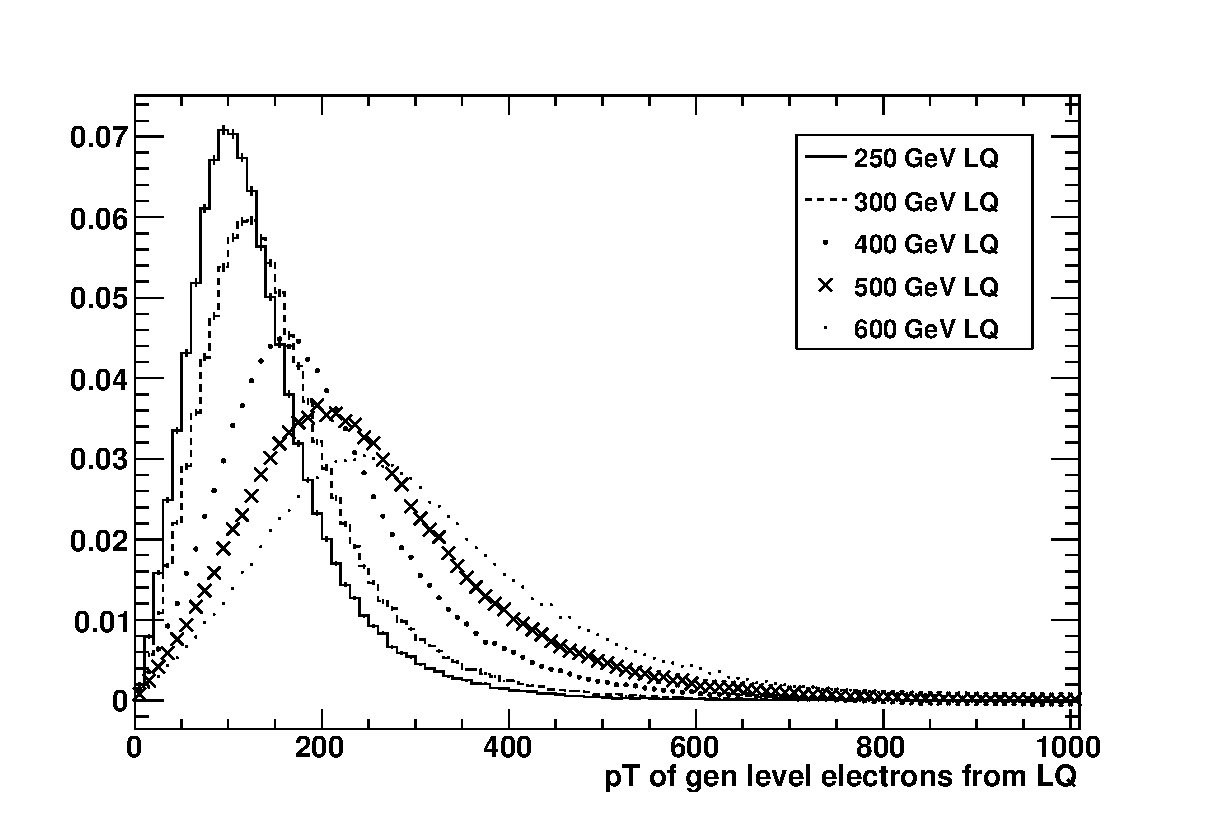
\includegraphics{plots/generatorLevel/GenElepT.eps}} &
  b.
  \resizebox{7.5cm}{!}{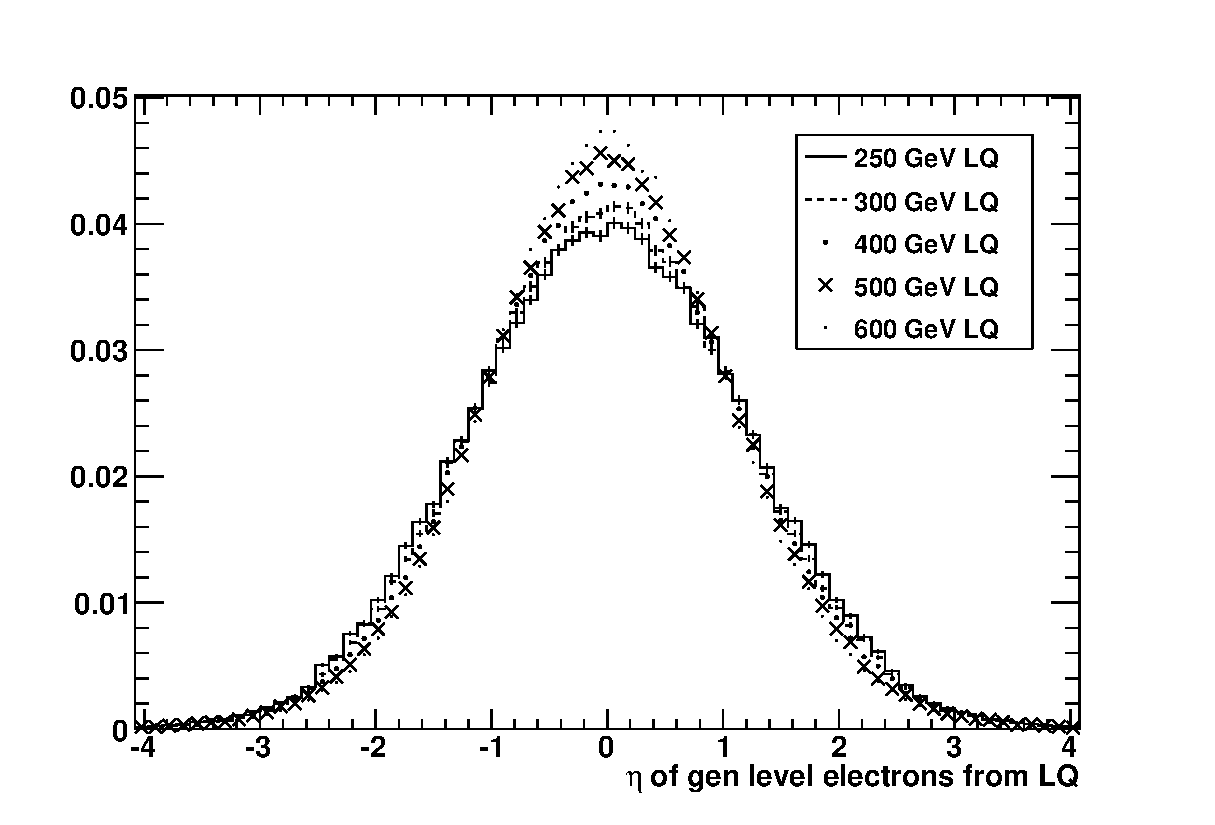
\includegraphics{plots/generatorLevel/GenEleEta.eps}} \\
  \end{tabular}
  \caption{\small \sl Distribution of the $P_t$ (a) and $\eta$ (b) variables at generator level for the electrons coming from the LQ decay.}
  \label{fig:genPlots}
  \end{center}
\end{figure}




%\end{document}
